\documentclass[tikz, border=10pt]{standalone}
\usepackage[T1]{fontenc}
\usepackage{mathpazo}
\usepackage{amsmath, amssymb}
\usetikzlibrary{positioning, arrows.meta, fit, backgrounds, calc, decorations.pathreplacing}

% Morandi palette
\definecolor{stblue}{HTML}{7B97AD}
\definecolor{sage}{HTML}{7A9A7E}
\definecolor{rwgold}{HTML}{B8995E}
\definecolor{terracotta}{HTML}{C47A6A}
\definecolor{lavender}{HTML}{907EA0}
\definecolor{cream}{HTML}{F9F6F0}
\definecolor{border}{HTML}{D4C9B8}
\definecolor{dkbrown}{HTML}{3D3530}
\definecolor{wmgray}{HTML}{7B7067}

% Lighter fills
\definecolor{sagelight}{HTML}{E4EDE5}
\definecolor{bluelight}{HTML}{DDE5EB}
\definecolor{goldlight}{HTML}{F0E6D3}
\definecolor{lavlight}{HTML}{E5DFE9}
\definecolor{terralight}{HTML}{F0DDD8}

\begin{document}
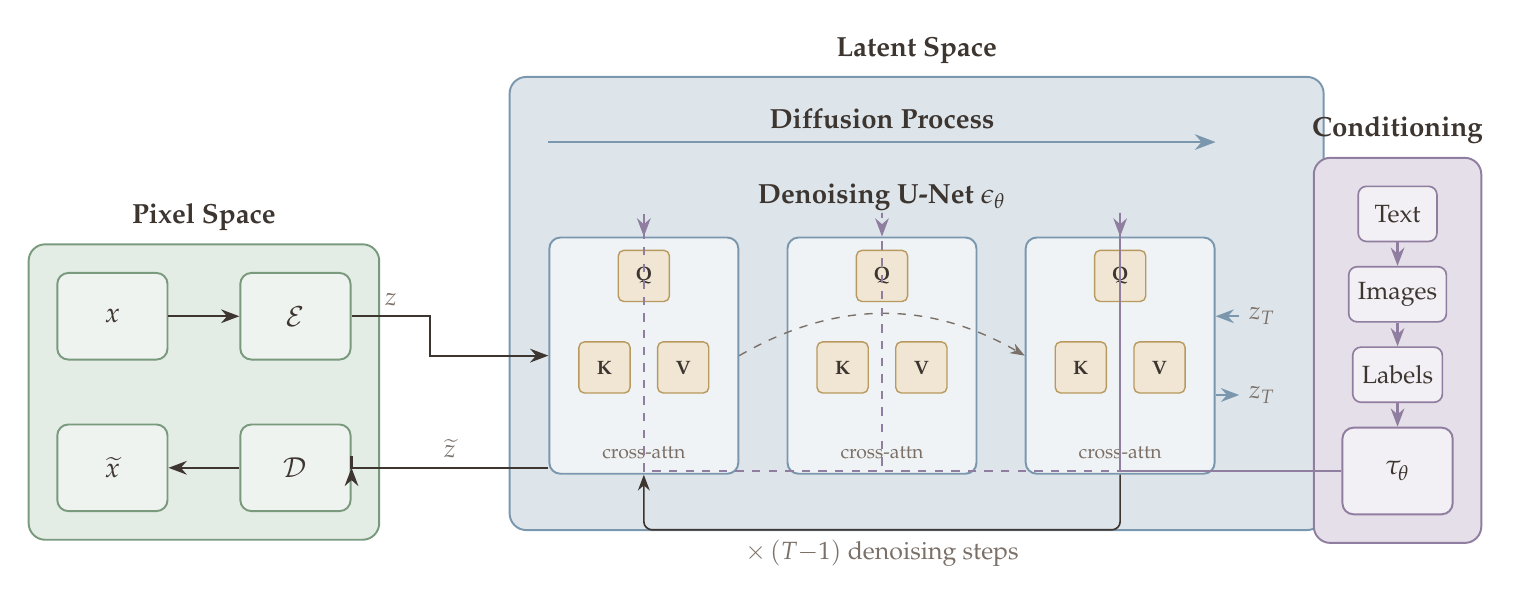
\begin{tikzpicture}[
  >=Stealth,
  node distance=0.6cm,
  every node/.style={font=\normalsize},
  block/.style={
    draw=#1, fill=#1!12, rounded corners=4pt,
    minimum height=1.1cm, minimum width=1.4cm,
    line width=0.7pt, font=\normalsize, text=dkbrown,
  },
  smallblock/.style={
    draw=#1, fill=#1!12, rounded corners=3pt,
    minimum height=0.7cm, minimum width=1.0cm,
    line width=0.6pt, font=\small, text=dkbrown,
  },
  qkv/.style={
    draw=rwgold, fill=goldlight, rounded corners=2pt,
    minimum height=0.55cm, minimum width=0.55cm,
    line width=0.5pt, font=\scriptsize\bfseries, text=dkbrown,
  },
  arr/.style={->, line width=0.8pt, dkbrown},
  darr/.style={<->, line width=0.8pt, dkbrown},
  label/.style={font=\small, text=wmgray},
  heading/.style={font=\normalsize\bfseries, text=dkbrown},
]

% === PIXEL SPACE (left) ===
\node[block=sage] (img) {$x$};
\node[block=sage, below=0.8cm of img] (imgout) {$\widetilde{x}$};

\node[block=sage, right=0.9cm of img] (enc) {$\mathcal{E}$};
\node[block=sage, right=0.9cm of imgout] (dec) {$\mathcal{D}$};

\draw[arr] (img) -- (enc);
\draw[arr] (dec) -- (imgout);

% Pixel space background
\begin{scope}[on background layer]
  \node[fit=(img)(imgout)(enc)(dec),
    fill=sagelight, draw=sage, rounded corners=6pt,
    line width=0.7pt, inner sep=10pt] (pixbox) {};
\end{scope}
\node[heading, above=1pt of pixbox.north] {Pixel Space};

% === LATENT SPACE (center) ===
% Latent codes
\node[right=1.0cm of enc] (z) {};
\node[right=1.0cm of dec] (ztilde) {};

% U-Net body
\node[right=1.8cm of enc, yshift=-0.5cm] (unetcenter) {};

% Denoising U-Net blocks (simplified as a row of cross-attention blocks)
\node[block=stblue, minimum width=2.4cm, minimum height=3.0cm,
  right=2.5cm of enc, yshift=-0.5cm] (unet1) {};
\node[block=stblue, minimum width=2.4cm, minimum height=3.0cm,
  right=0.6cm of unet1] (unet2) {};
\node[block=stblue, minimum width=2.4cm, minimum height=3.0cm,
  right=0.6cm of unet2] (unet3) {};

% Q K V labels inside each U-Net block
\foreach \blk in {unet1, unet2, unet3} {
  \node[qkv, minimum height=0.65cm, minimum width=0.65cm]
    at ($(\blk.north)+(0,-0.5)$) {Q};
  \node[qkv, minimum height=0.65cm, minimum width=0.65cm]
    at ($(\blk.center)+(-0.5,-0.15)$) {K};
  \node[qkv, minimum height=0.65cm, minimum width=0.65cm]
    at ($(\blk.center)+(0.5,-0.15)$) {V};
}

% Cross-attention label
\node[font=\scriptsize, text=wmgray] at ($(unet1.south)+(0,0.28)$) {cross-attn};
\node[font=\scriptsize, text=wmgray] at ($(unet2.south)+(0,0.28)$) {cross-attn};
\node[font=\scriptsize, text=wmgray] at ($(unet3.south)+(0,0.28)$) {cross-attn};

% U-Net label
\node[heading] at ($(unet2.north)+(0,0.5)$) {Denoising U-Net $\epsilon_\theta$};

% Diffusion process arrow above
\node[above=1.2cm of unet1.north west, anchor=west] (diffleft) {};
\node[above=1.2cm of unet3.north east, anchor=east] (diffright) {};
\draw[arr, line width=1pt, stblue] (diffleft.west) -- node[above, heading, yshift=1pt] {Diffusion Process} (diffright.east);

% Skip connections (curved lines between blocks)
\draw[arr, dashed, wmgray, line width=0.5pt, bend left=30] (unet1.east) to (unet3.west);

% z arrow from encoder to U-Net
\draw[arr] (enc.east) -- ++(0.5,0) node[above, label] {$z$} -- ++(0.5,0) |- (unet1.west);

% z̃ arrow from U-Net to decoder
\draw[arr] (unet1.west |- dec) -| (dec.east |- dec) ;
\path (unet1.west |- dec) -- (dec.east) node[midway, above, label] {$\widetilde{z}$};

% z_T label on right side
\node[right=0.3cm of unet3, label, yshift=0.5cm] (zt) {$z_T$};
\node[right=0.3cm of unet3, label, yshift=-0.5cm] (zt2) {$z_T$};
\draw[arr, stblue] (zt) -- (unet3.east |- zt);
\draw[arr, stblue] (unet3.east |- zt2) -- (zt2);

% Iterative denoising loop
\draw[arr, dkbrown, line width=0.6pt, rounded corners=3pt]
  (unet3.south) -- ++(0,-0.7) -| (unet1.south)
  node[pos=0.25, below, font=\small, text=wmgray] {$\times\,(T{-}1)$ denoising steps};

% Latent space background
\begin{scope}[on background layer]
  \node[fit=(diffleft)(diffright)(unet1)(unet2)(unet3)(zt)(zt2),
    fill=bluelight, draw=stblue, rounded corners=6pt,
    line width=0.7pt, inner xsep=14pt, inner ysep=20pt] (latbox) {};
\end{scope}
\node[heading, above=1pt of latbox.north] {Latent Space};

% === CONDITIONING (right) ===
\node[smallblock=lavender, right=1.8cm of unet3, yshift=1.8cm] (ctext) {Text};
\node[smallblock=lavender, below=0.3cm of ctext] (cimg) {Images};
\node[smallblock=lavender, below=0.3cm of cimg] (csem) {Labels};

% tau_theta
\node[block=lavender, below=0.3cm of csem, minimum width=1.4cm] (tau) {$\tau_\theta$};

\draw[arr, lavender] (ctext.south) -- (ctext |- cimg.north);
\draw[arr, lavender] (cimg.south) -- (cimg |- csem.north);
\draw[arr, lavender] (csem.south) -- (csem |- tau.north);

% Conditioning arrows into U-Net cross-attention
\draw[arr, lavender, line width=0.8pt] (tau.west) -| ($(unet3.north)+(0,0.3)$) -- (unet3.north);
\draw[arr, lavender, line width=0.8pt, dashed] (tau.west) -| ($(unet2.north)+(0,0.3)$) -- (unet2.north);
\draw[arr, lavender, line width=0.8pt, dashed] (tau.west) -| ($(unet1.north)+(0,0.3)$) -- (unet1.north);

% Conditioning background
\begin{scope}[on background layer]
  \node[fit=(ctext)(cimg)(csem)(tau),
    fill=lavlight, draw=lavender, rounded corners=6pt,
    line width=0.7pt, inner sep=10pt] (condbox) {};
\end{scope}
\node[heading, above=1pt of condbox.north] {Conditioning};

\end{tikzpicture}
\end{document}
